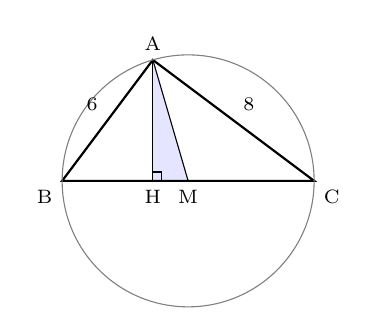
\begin{tikzpicture}[scale=0.32]
\fill[blue!10] (3.600,4.800)--(3.600,0.000)--(5.000,0.000)--cycle;\draw[thick] (3.600,4.800)--(0.000,0.000)--(10.000,0.000)--cycle; \draw (3.600,4.800)--(3.600,0.000); \draw (3.600,4.800)--(5.000,0.000); \draw[gray] (5,0) circle (5);\draw (3.6,0.35)--(3.95,0.35)--(3.95,0);\fill (3.600,0.000) circle (1.5pt);\fill (5.000,0.000) circle (1.5pt);\node[above] at (3.600,4.800){\scriptsize A};\node[below left] at (0.000,0.000){\scriptsize B};\node[below right] at (10.000,0.000){\scriptsize C};\node[below] at (3.600,0.000){\scriptsize H};\node[below] at (5.000,0.000){\scriptsize M};\node[above left] at (1.800,2.400){\scriptsize 6};\node[above right] at (6.800,2.400){\scriptsize 8};
\end{tikzpicture}